\documentclass{article}
\usepackage{fullpage}
\usepackage[]{amsmath}
\usepackage[]{siunitx}
\usepackage[]{gensymb}
\usepackage[]{steinmetz}
\usepackage[]{chngcntr}
\usepackage[]{dsfont}
\usepackage[]{hyperref}
\usepackage[]{xcolor}
\usepackage[]{float}
\usepackage[final]{pdfpages}
\usepackage[]{calculator}
\hypersetup{
    colorlinks,
    linkcolor={blue!50!black},
    citecolor={blue!50!black}
}
\numberwithin{equation}{section}
\renewcommand{\thesection}{}
\renewcommand{\thesubsection}{}
\renewcommand{\thesubsubsection}{}
\renewcommand{\theequation}{\thesection\arabic{equation}}
\makeatletter
\def\@seccntformat#1{\csname #1ignore\expandafter\endcsname\csname the#1\endcsname\quad}
\let\sectionignore\@gobbletwo
\let\latex@numberline\numberline
\def\numberline#1{\if\relax#1\relax\else\latex@numberline{#1}\fi}
\makeatother
\title{ECE 671 Fall 2015 Assignment 3}
\author{John Rinehart}
\date{\today}

\begin{document}
\maketitle
\tableofcontents
\section*{Foreword}

This problem set had me using a few tools at different times. I used Keysight's
Advanced Design Suite (ADS) at a few points during my homework, for simulations.
I have also used Mathematica, extensively, to assist me with algebra and
plugging in values. Each problem is more or less self-contained in the written
text. However, if you want to see calculations or simulations of anything that
is referenced in the problem please consult the appendix for the associated
problem. I have almost as many appendices as problems to account for this extra
information. Please don't hesitate to ask me any questions you may have
concerning my work. I have done my best to make it clear, but sometimes clear is
only ``clear'' to one's self.

\section{Problem 1a: High Gain Amplifier}
\label{sec:A2P1}

\subsection{Ideal Biasing Network}
In accordance with the text delivered in the \hyperref[sec:Foreword]{Foreword}
the ideal design is given below. I have simulated the scattering parameters
according the schematic (biasing) shown in figure
\ref{fig:A2P1IdealSchematic}.

\begin{figure}[H]
    \centering
    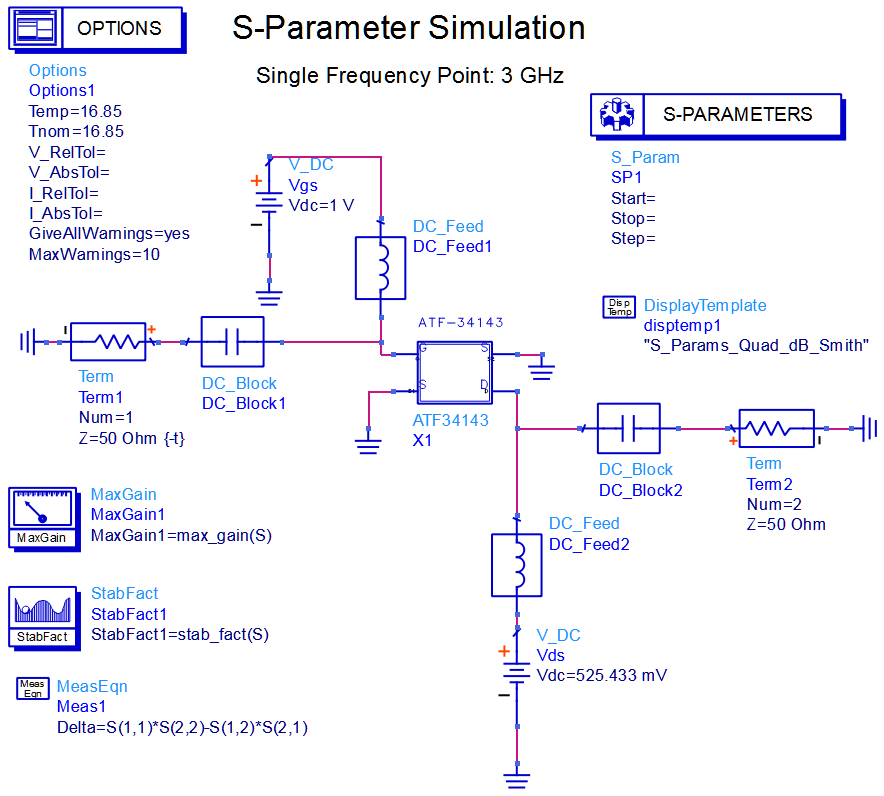
\includegraphics[width=0.8\linewidth]{Images/A2P1IdealSchematic.png}
    \caption{Schematic of the biasing network for the high-gain amplifier}
    \label{fig:A2P1IdealSchematic}
\end{figure}

The results of simulating this biasing network are given in figure
\ref{fig:A2P1IdealBiasingResults}. Note that the transistor is stable in that $K
>1$ and $|\Delta < 1$. Hand calculations that confirm this are given in the
appendix (Mathematica).

\begin{figure}[H]
    \centering
    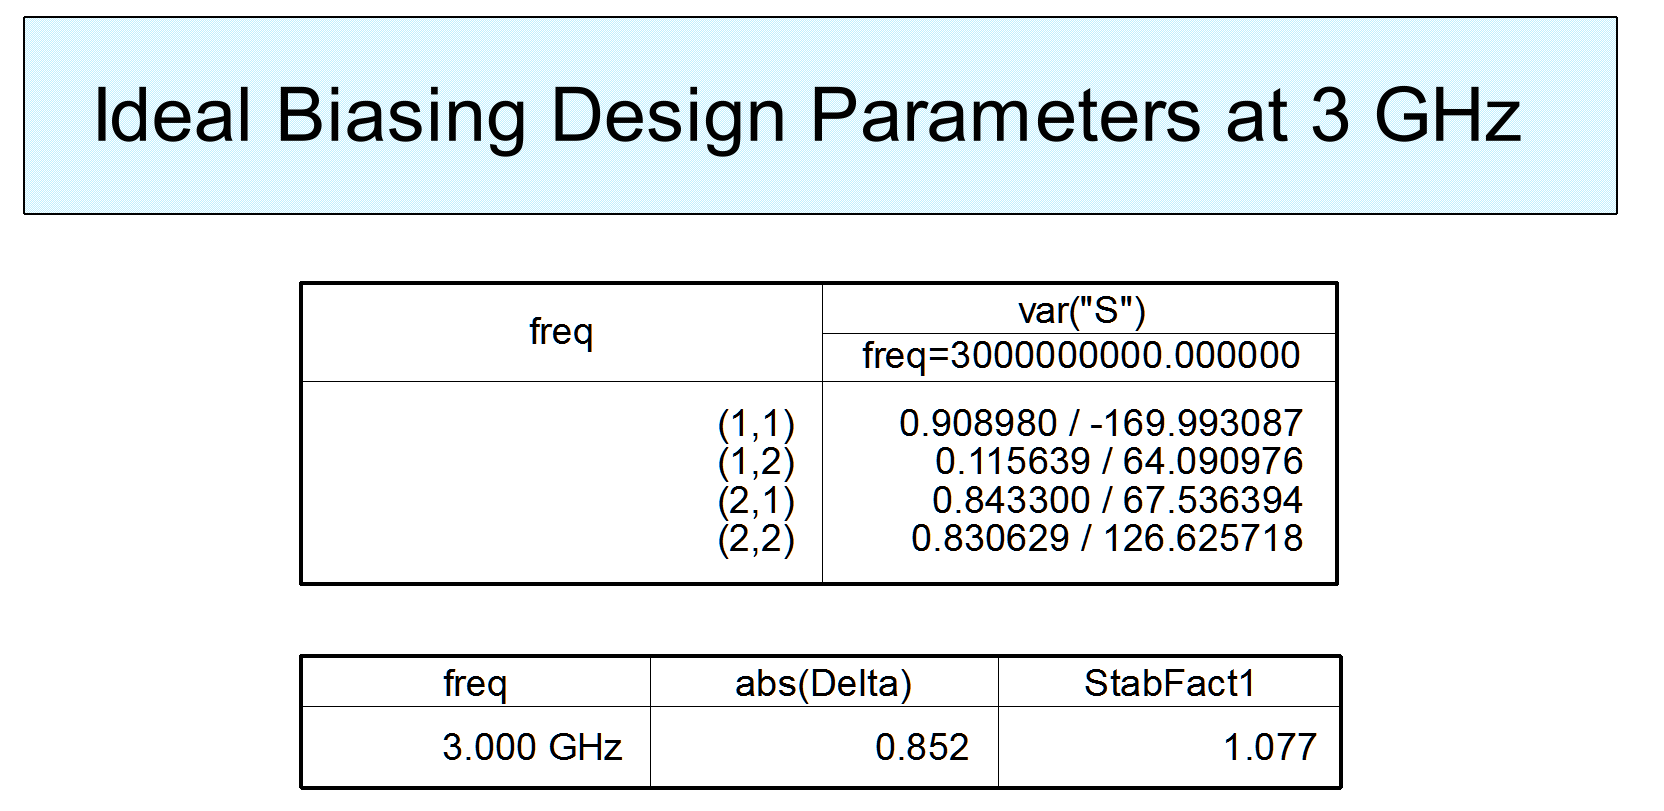
\includegraphics[width=0.8\linewidth]{Images/A2P1IdealBiasingResults}
    \caption{Results of simulating the biasing network shown in figure
    \ref{fig:A2P1IdealSchematic}}
    \label{fig:A2P1IdealBiasingResults}
\end{figure}

\subsection{Physical Biasing Network}
If I replace the DC feeds (ideal inductors) and DC blocks (ideal capacitors)
with the following values I obtain the following schematic and results:

\begin{figure}[H]
    \centering
    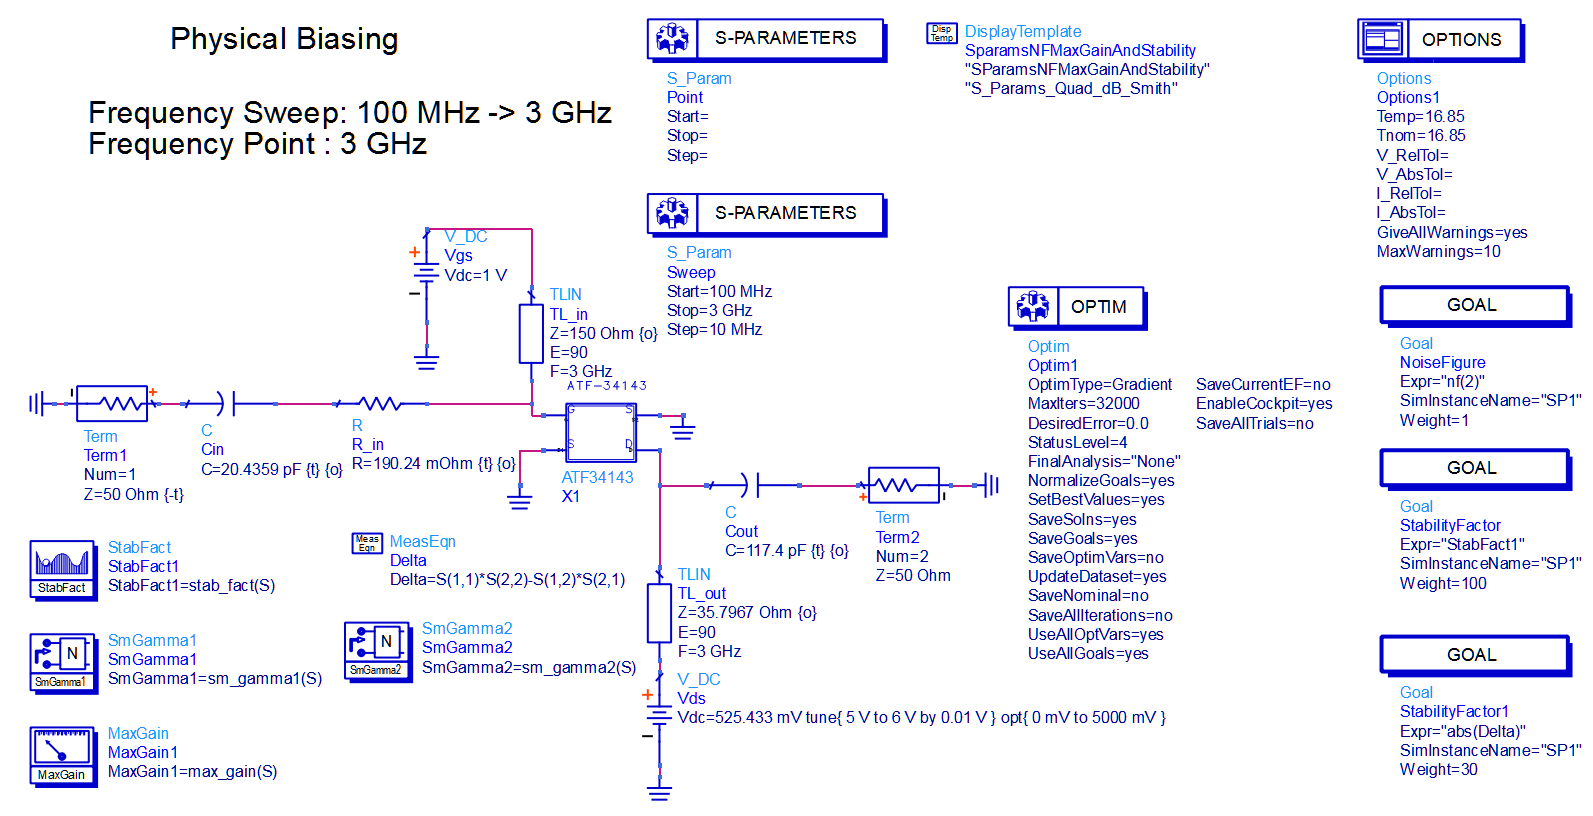
\includegraphics[width=0.8\linewidth]{Images/A2P1PhysicalSchematic.png}
    \caption{High-gain amplifier biasing network using real components}
    \label{fig:A2P1PhysicalSchematic}
\end{figure}

\begin{figure}[H]
    \centering
    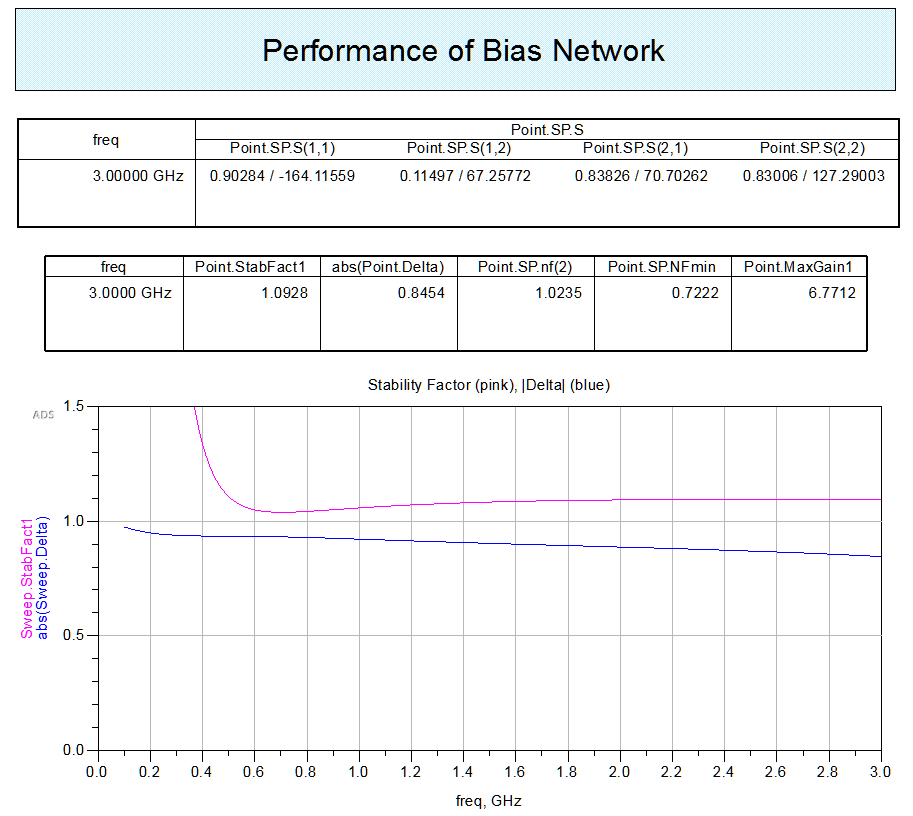
\includegraphics[width=0.8\linewidth]{Images/A2P1PhysicalBiasingResults.png}
    \caption{Real-component biasing results for the high-gain amplifier.}
    \label{fig:A2P1PhysicalBiasingResults}
\end{figure}

Note that while $G_{T_{max}}$ is included, here, in the simulated data
$\Gamma_{ms}$ and $\Gamma_{ml}$ have not been simulated. Instead, hand
calculations have been done to determine these quantities. The calculated values
can be found in the Mathematica code in the appendix.

In the appendix I also relate the physical network to the ideal network. There,
I also include the MATTLAB code that I have used to relate the scattering parameters
obtained by simulating the ideal biasing to that of the network comprising the
physical components. Note that while it is known that short transmission lines
of low impedance behave like inductors, the transmission lines used to couple
$V_{gs}$ and $V_{ds}$ to the amplifier suffice even though they are not
sufficiently short or sufficiently low in impedance to qualify as inductors.
This was a design choice. Below, I include a table for easy comparison that
relates the values of $S_{11}, S_{12}, S_{21}, S_{22}$ obtained using a
simulation with the values obtained using MATLAB.

\begin{center}
    \begin{tabular}{|c|c|c|}
        \hline Scattering Parameter & ADS Value & ``Hand-calculated'' MATLAB values \\
        \hline $S_{11}$ & .90284 \phase{-164.12 \degree} & .90283
        \phase{-164.12 \degree} \\
        \hline $S_{12}$ & .11497 \phase{67.257 \degree} & .11495 \phase{67.257
    \degree}\\
        \hline $S_{21}$ & .83826 \phase{70.703 \degree} & .83838 \phase{70.702
\degree} \\
        \hline $S_{22}$ & .83006 \phase{127.29 \degree}  & .83003 \phase{127.29
        \degree} \\ \hline
    \end{tabular}
\end{center}

Note that the stability of the transistor at the design frequency was also
assessed using ADS. ``Hand calculations'' of the Rollett stability factor as
well as the determinant of the scattering parameter matrix are given in the
appendix. They do not differ significantly from the ADS values (they are within
numerical error: a part in ten thousand) so they have not been included here.

Since the transistor is unconditionally stable at the design frequency ($K >1$
and $|\Delta|<1$) no shunting resistor will be used to stabilize the device.

\subsection{Full Design: A High-Gain Amplifier}

The last thing to do is insert a matching network that accomplishes the goal of
the design: To deliver more power to the load. According to the design
requirements, the matching network must be such that $G_{T_{max}} - G_t \le 1$.
A bonus feature that the customer is requiring is the lowest noise figure as is possible
given some transducer gain, $G_t > G_{T_{max}} -1$. However, no lower bound is placed on the
values of $G_{T_{max}}$. So, given that there is always a trade-off in amplifier
design between transducer gain and noise figure it makes sense to reduce the
noise figure to something sufficiently low while keeping the gain
``sufficiently'' high. Granted, the \SI{6}{\deci\bel} of transducer gain
provided by this design is not great.  However, the noise figure is very low ($<
\SI{1}{\deci\bel}$) which was prioritized over the forward gain.

The design of the amplifier is given below in figure
\ref{fig:A2P1AmplifierSchematic}. The results are given below in figures
\ref{fig:A2P1AmplifierDesignFrequencyEfficacy},\ref{fig:A2P1AmplifierFrequencySweepStability},\ref{fig:A2P1AmplifierFOM}.

Note the addition of the series resistor at the input to the gate of the
amplifier. This was used to stabilize the transistor over the specified $
\SI{100}{\mega\hertz} \rightarrow \SI{3}{\giga\hertz}$ bandwidth.

\begin{figure}[H]
    \centering
    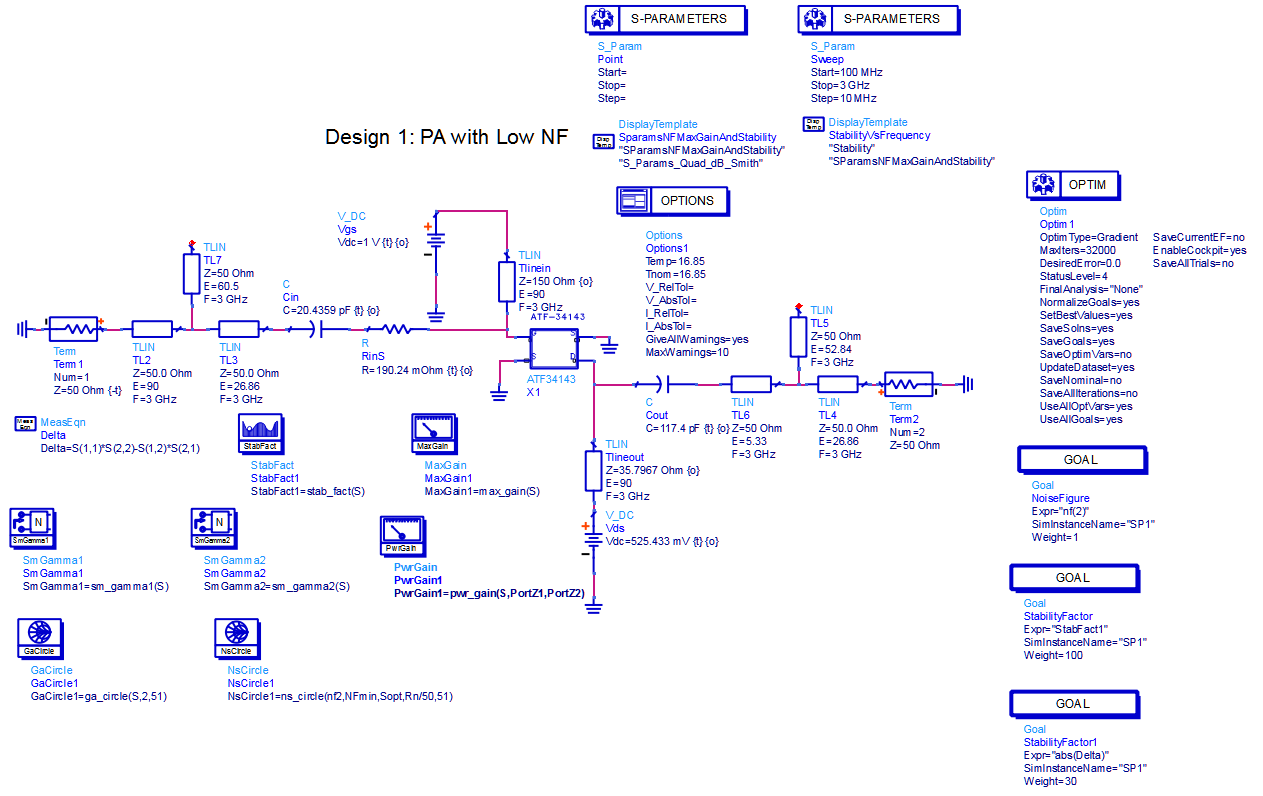
\includegraphics[width=0.8\linewidth]{Images/A2P1AmplifierSchematic.png}
    \caption{Schematic of the high gain amplifier}
    \label{fig:A2P1AmplifierSchematic}
\end{figure}

\begin{figure}[H]
    \centering
    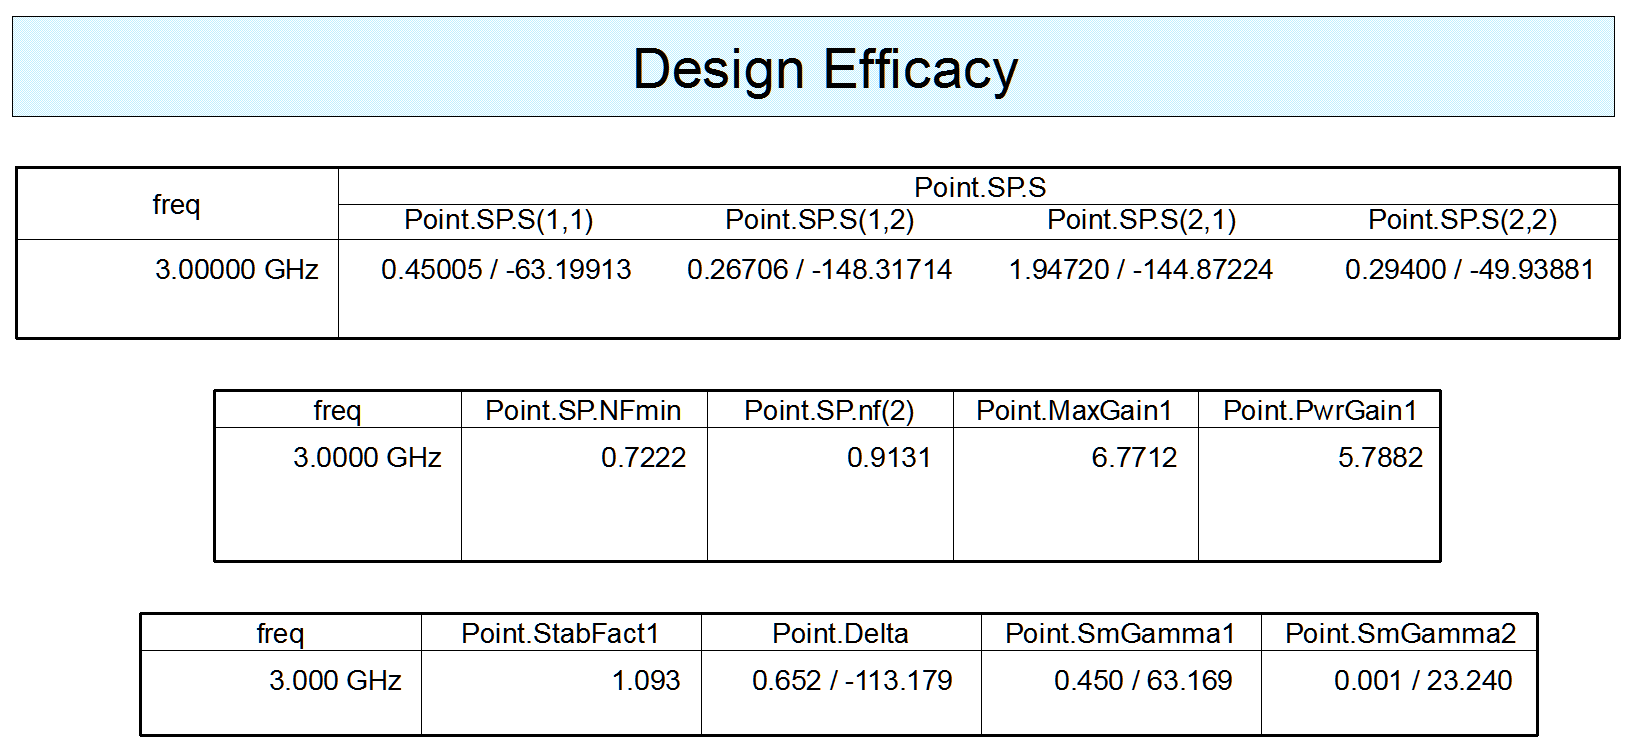
\includegraphics[width=0.8\linewidth]{Images/A2P1AmplifierDesignFrequencyEfficacy.png}
    \caption{Efficacy of the amplifier at the design frequency}
    \label{fig:A2P1AmplifierDesignFrequencyEfficacy}
\end{figure}

\begin{figure}[H]
    \centering
    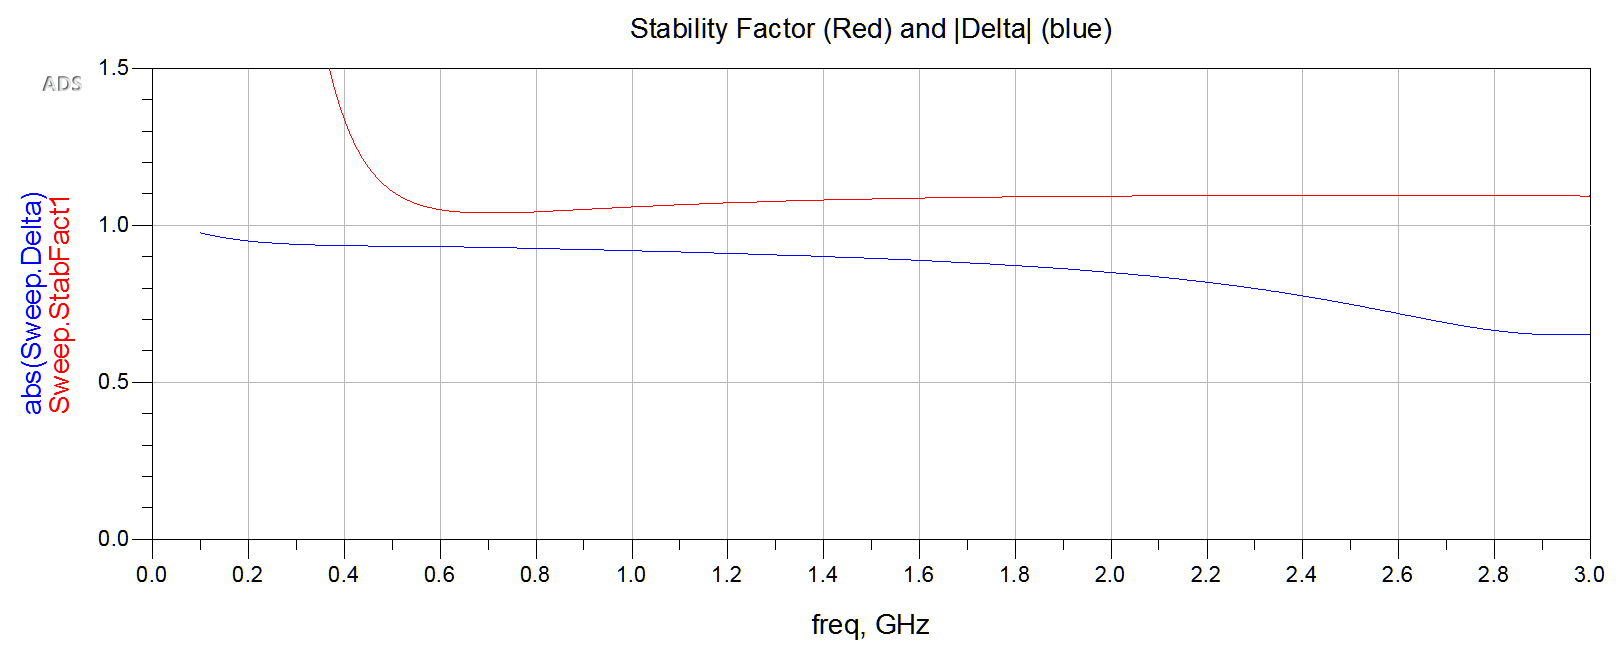
\includegraphics[width=0.8\linewidth]{Images/A2P1AmplifierFrequencySweepStability.png}
    \caption{Stability of the amplifier over the required bandwidth}
    \label{fig:A2P1AmplifierFrequencySweepStability}
\end{figure}

\begin{figure}[H]
    \centering
    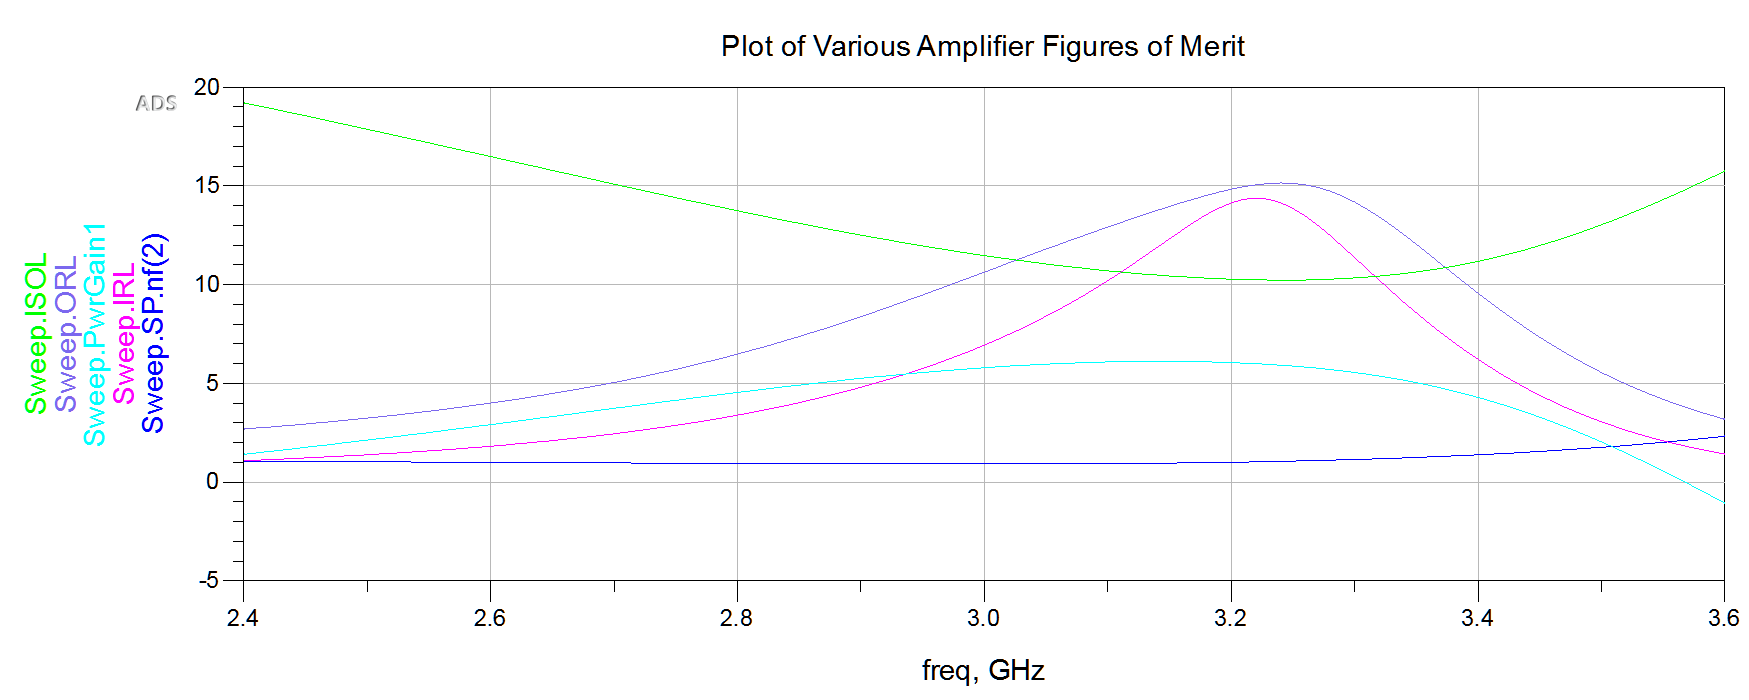
\includegraphics[width=0.8\linewidth]{Images/A2P1AmplifierFOM.png}
    \caption{Plot of various figures of merit of the amplifier including:
    Isolation (green), output return loss (purple), power gain (teal), input
return loss (pink) and noise figure (blue)}
    \label{fig:A2P1AmplifierFOM}
\end{figure}

A few notes regarding the design of the amplifier. It has already been noted
that the gain is not as high as could be attained with this transistor ($\approx
\SI{18}{\deci\bel}$) but noise figure was prioritized. Furthermore, you may
notice that terminal 1 is not matched to the rest of the amplifier circuit
($\Gamma_{ms} \approx .45 \phase{63 \degree} \ne 0$). This was intentional.
Introducing mismatch allowed the noise figure to be reduced even more than it
had been while sacrificing some performance in gain ($ G_T \ne G_{T_{max}}$).
Note that the gain is still within the specified distance from $G_{t_{max}}$ in
that $G_{T_{max}} - G_T \approx \SI{.993}{\deci\bel}$.

\section{Low Noise Figure Amplifier}

\subsection{Ideal Biasing}

In a similar manner as with the high gain amplifier I include below, in figures
\ref{fig:A2P2IdealSchematic} and \ref{fig:A2P2IdealBiasingResult:},
respectively, the schematic and the results (scattering parameters and
stability) of the simulation at the design frequency (\SI{2}{\giga\hertz}).

\begin{figure}[H]
    \centering
    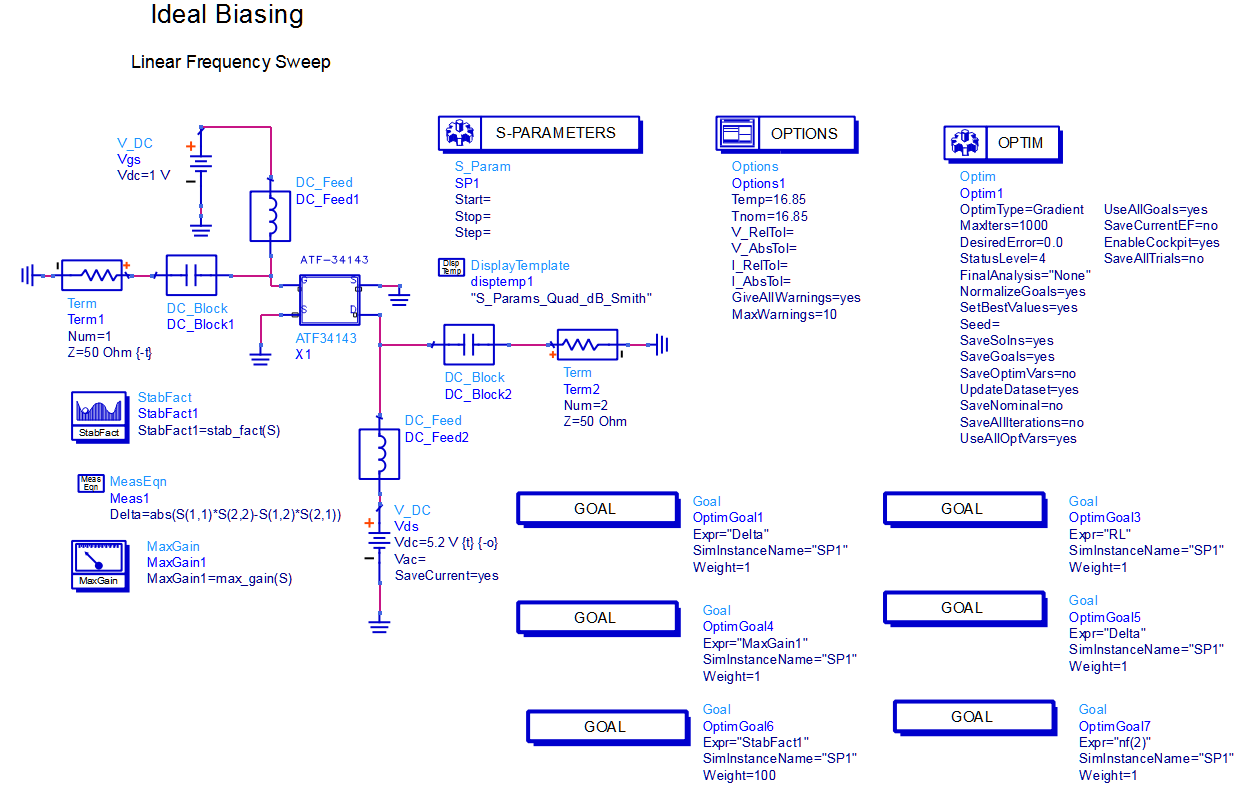
\includegraphics[width=0.8\linewidth]{Images/A2P2IdealSchematic.png}
    \caption{Schematic of the low noise amplifier ideal biasing network}
    \label{fig:A2P2IdealSchematic}
\end{figure}

\begin{figure}[H]
    \centering
    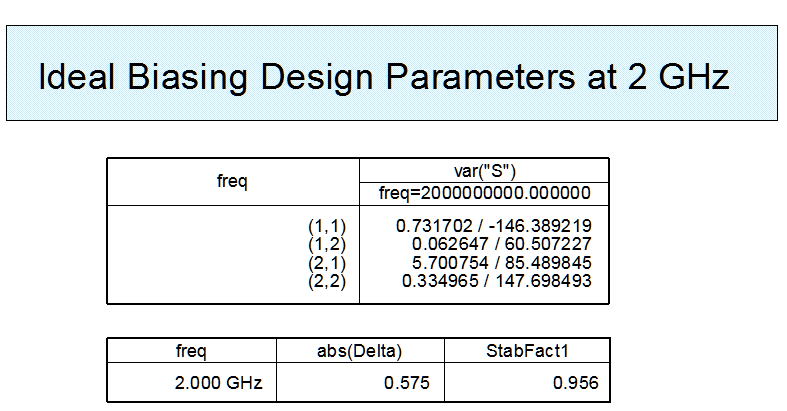
\includegraphics[width=0.8\linewidth]{Images/A2P2IdealBiasingResults.png}
    \caption{Results of the ADS simulation of the low noise amplifier ideal biasing network}
    \label{fig:A2P2IdealBiasingResults}
\end{figure}

\subsection{Physical Biasing}

The schematic and the simulation results of the physical biasing network for the
low noise amplifier are shown in figures \ref{fig:A2P2PhysicalSchematic} and
\ref{fig:A2P2PhysicalResults}, respectively.

Worthy of note: 
\begin{enumerate}
    \item   Figure \ref{fig:A2P2PhysicalResults} indicates stability over the
        entire bandwidth of consideration.
    \item   The return loss is given as $\approx \SI{3.1E-4}{\deci\bel}$.
    \item   The maximum gain at the noise figure selected, $\approx
        \SI{.88}{\deci\bel}$, manages to be quite high at $\SI{2}{\giga\hertz}$:
        $\approx \SI{16.8}{\deci\bel}$.
\end{enumerate}

\begin{figure}[H]
    \centering
    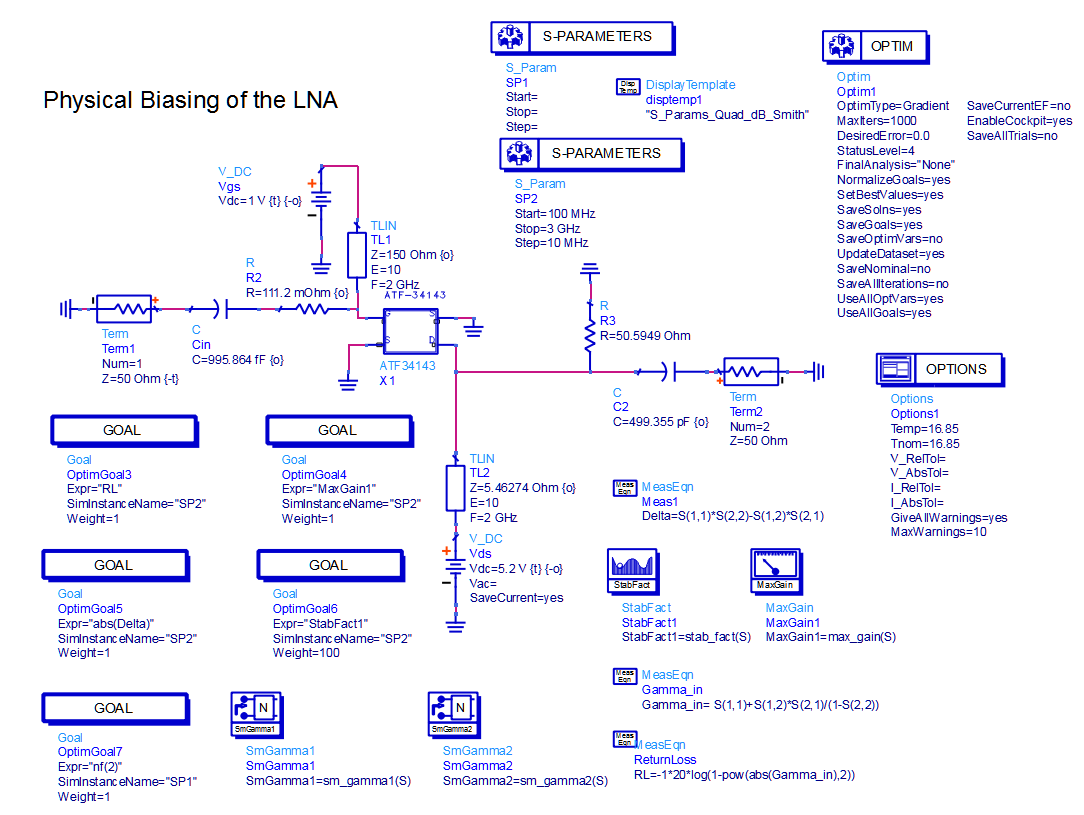
\includegraphics[width=0.8\linewidth]{Images/A2P2PhysicalSchematic.png}
    \caption{Schematic of the physical biasing network for the low noise
    amplifier.}
    \label{fig:A2P2PhysicalSchematic}
\end{figure}

\begin{figure}[H]
    \centering
    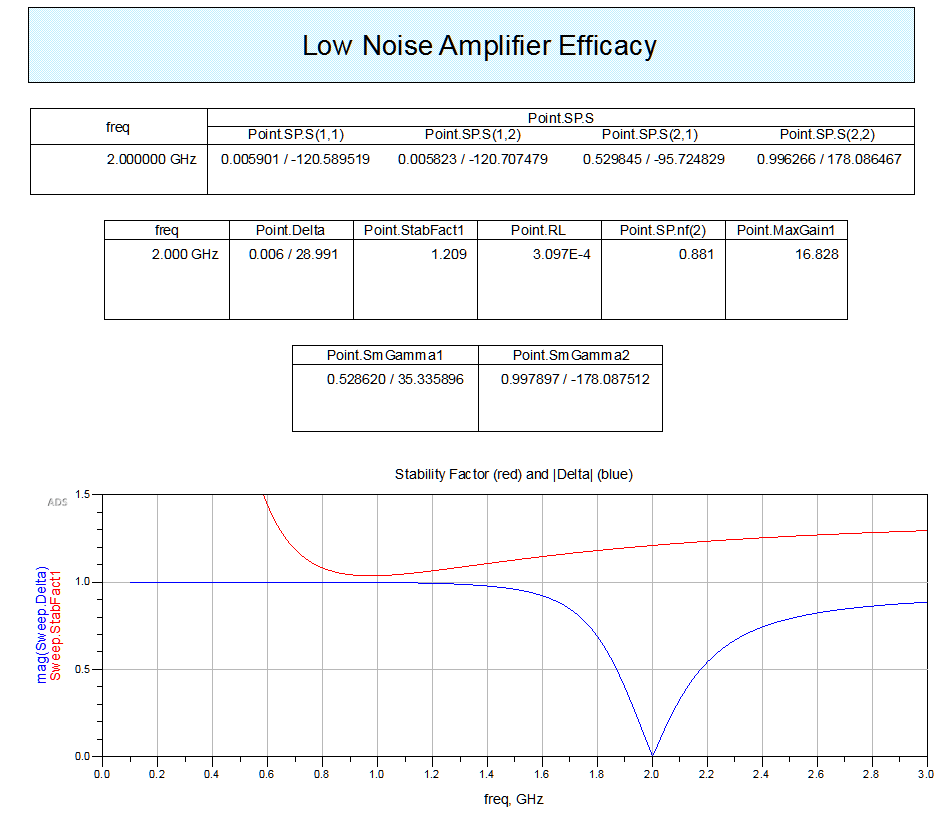
\includegraphics[width=0.8\linewidth]{Images/A2P2PhysicalResults.png}
    \caption{Efficacy of the low-noise amplifier physical biasing network. Note
    the extremely low designed return loss.}
    \label{fig:A2P2PhysicalResults}
\end{figure}

\subsection{Low Noise Amplifier Design}

The full design for the low noise amplifier is shown in figure
\ref{fig:A2P2LNASchematic}. The design efficacy is demonstrated in figures
\ref{fig:A2P2LNADesignFrequencyEfficacy},
\ref{fig:A2P2LNAFrequencySweepStability} and \ref{fig:A2P2LNAFOM}.

\begin{figure}[H]
    \centering
    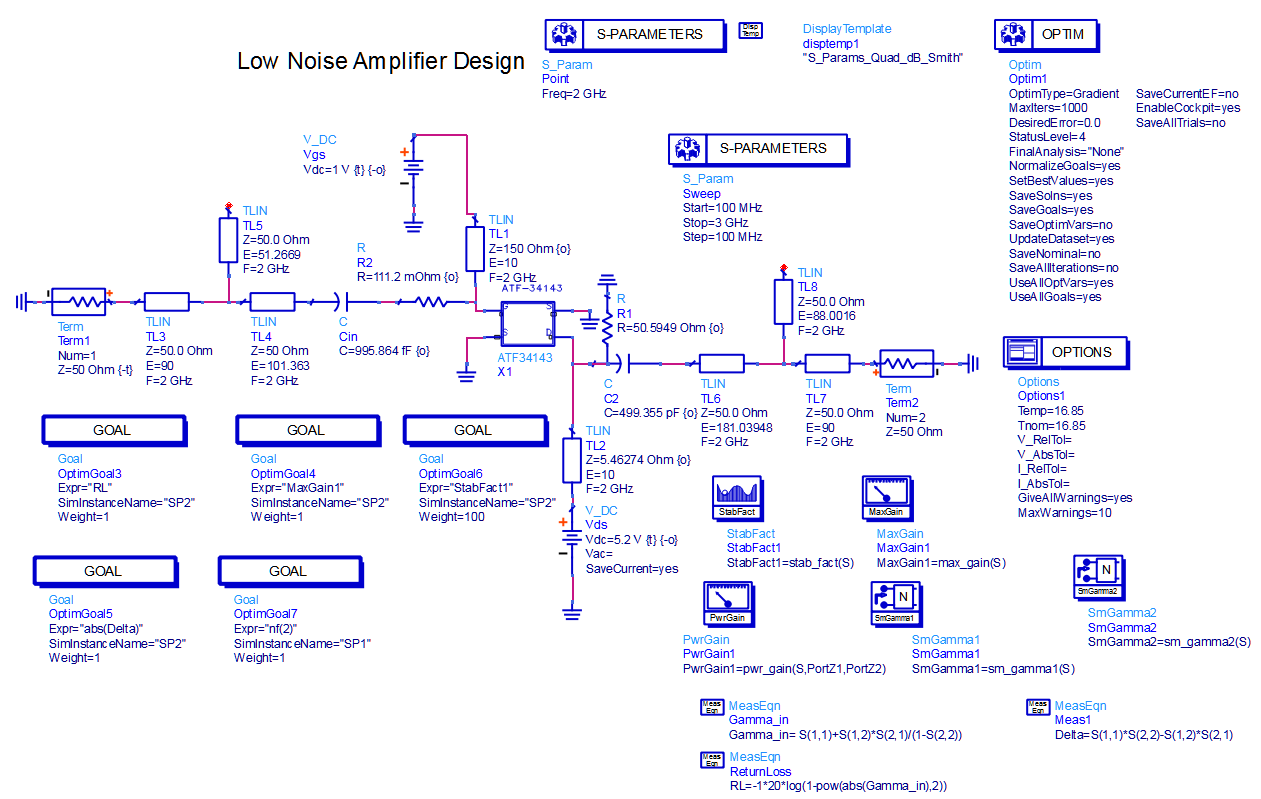
\includegraphics[width=0.8\linewidth]{Images/A2P2LNASchematic.png}
    \caption{Schematic of the LNA design.}
    \label{fig:A2P2LNASchematic}
\end{figure}

\begin{figure}[H]
    \centering
    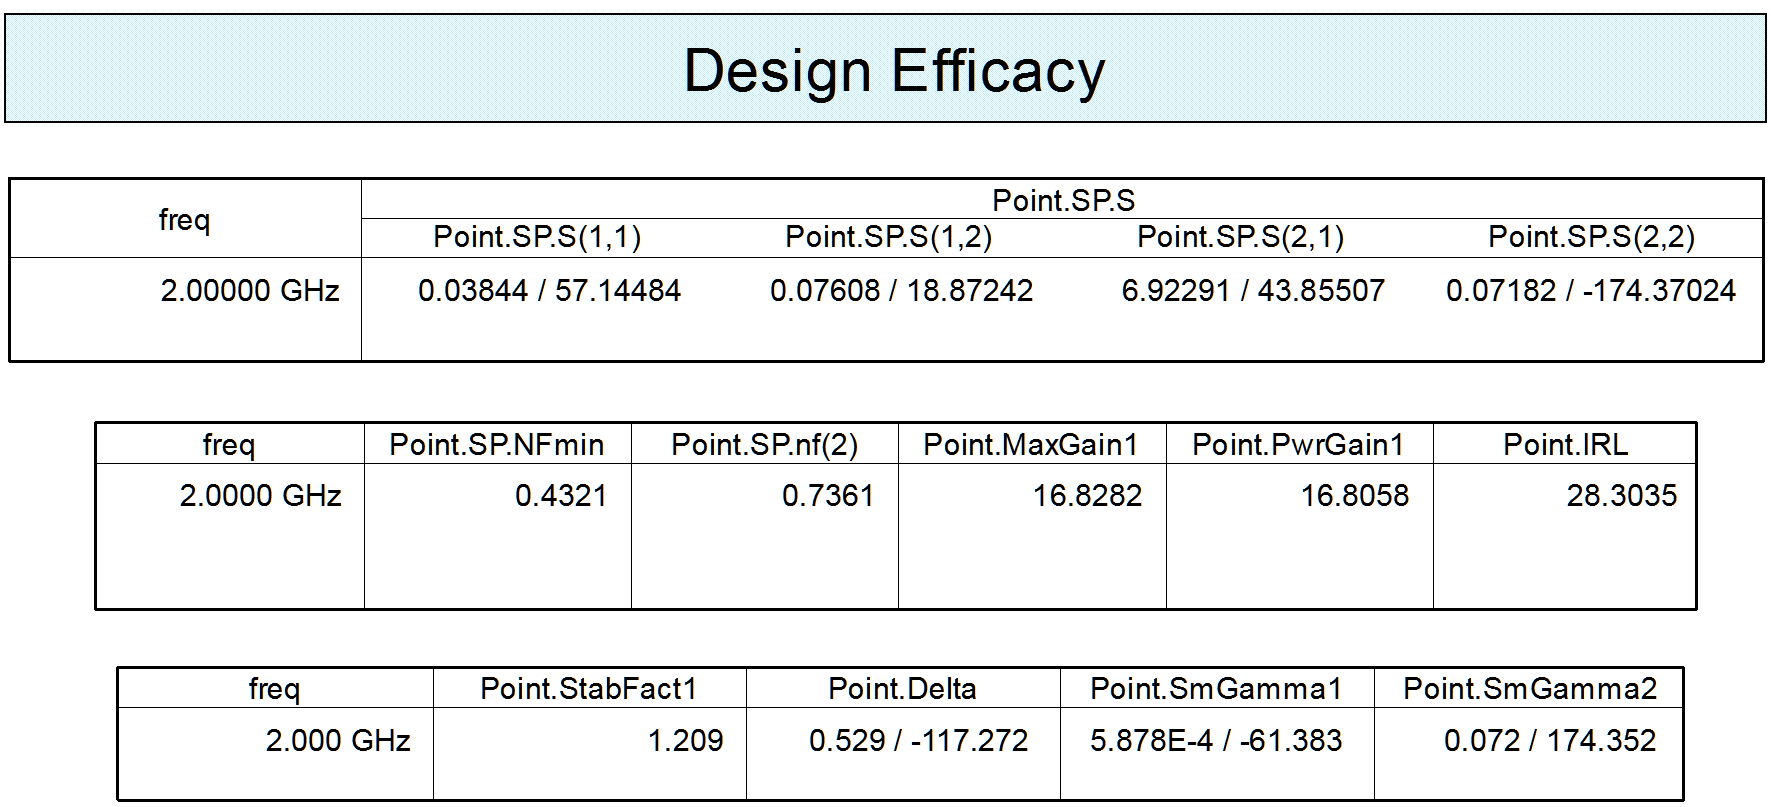
\includegraphics[width=0.8\linewidth]{Images/A2P2LNADesignFrequencyEfficacy.png}
    \caption{LNA efficacy at the design frequency: $\SI{2}{\giga\hertz}$.}
    \label{fig:A2P2LNADesignFrequencyEfficacy}
\end{figure}

\begin{figure}[H]
    \centering
    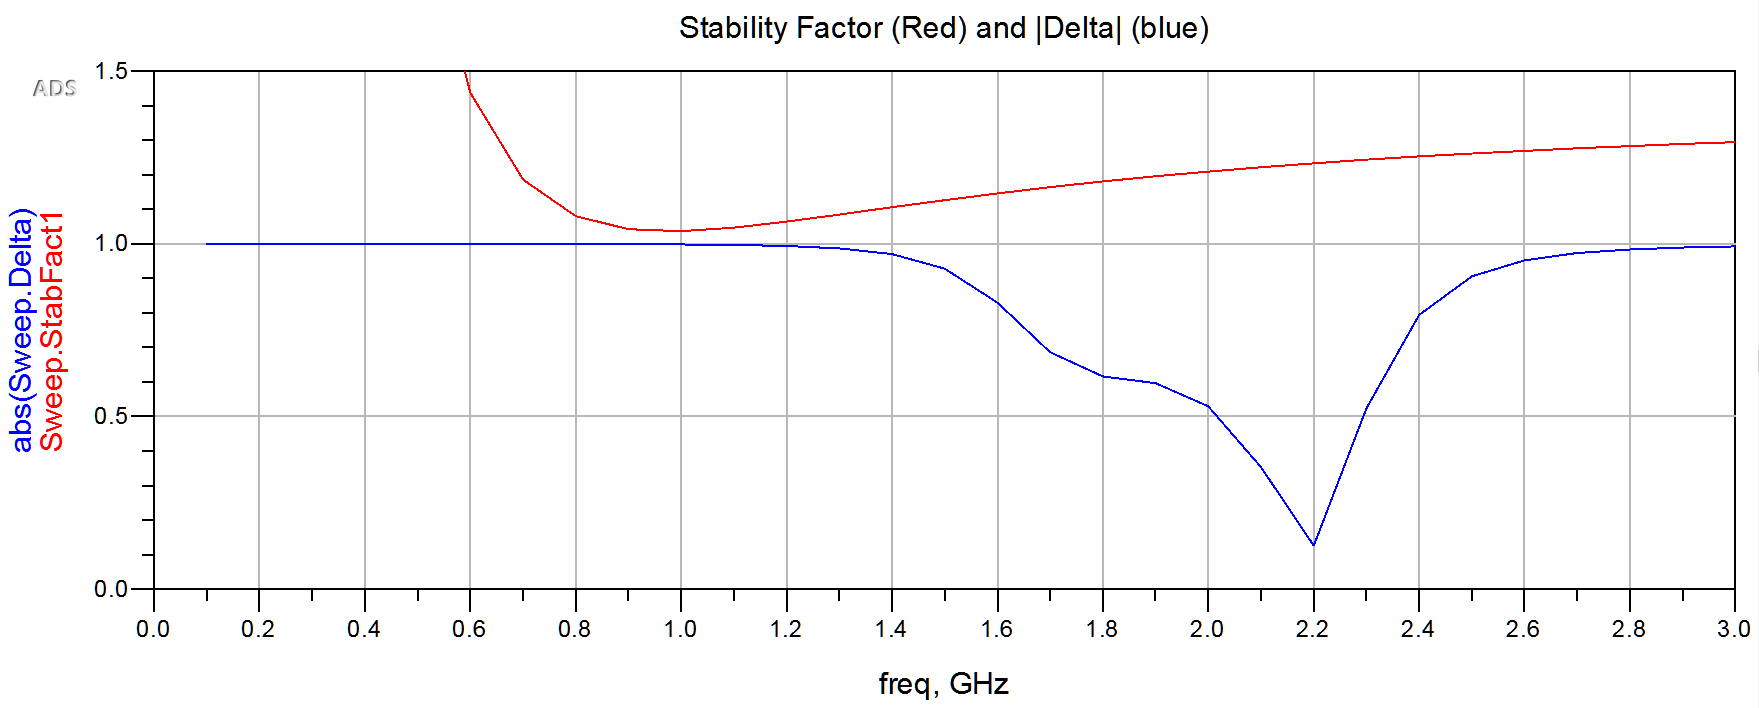
\includegraphics[width=0.8\linewidth]{Images/A2P2LNAFrequencySweepStability.png}
    \caption{LNA stability over the specified bandwidth of the amplifier.}
    \label{fig:A2P2LNAFrequencySweepStability}
\end{figure}

\begin{figure}[H]
    \centering
    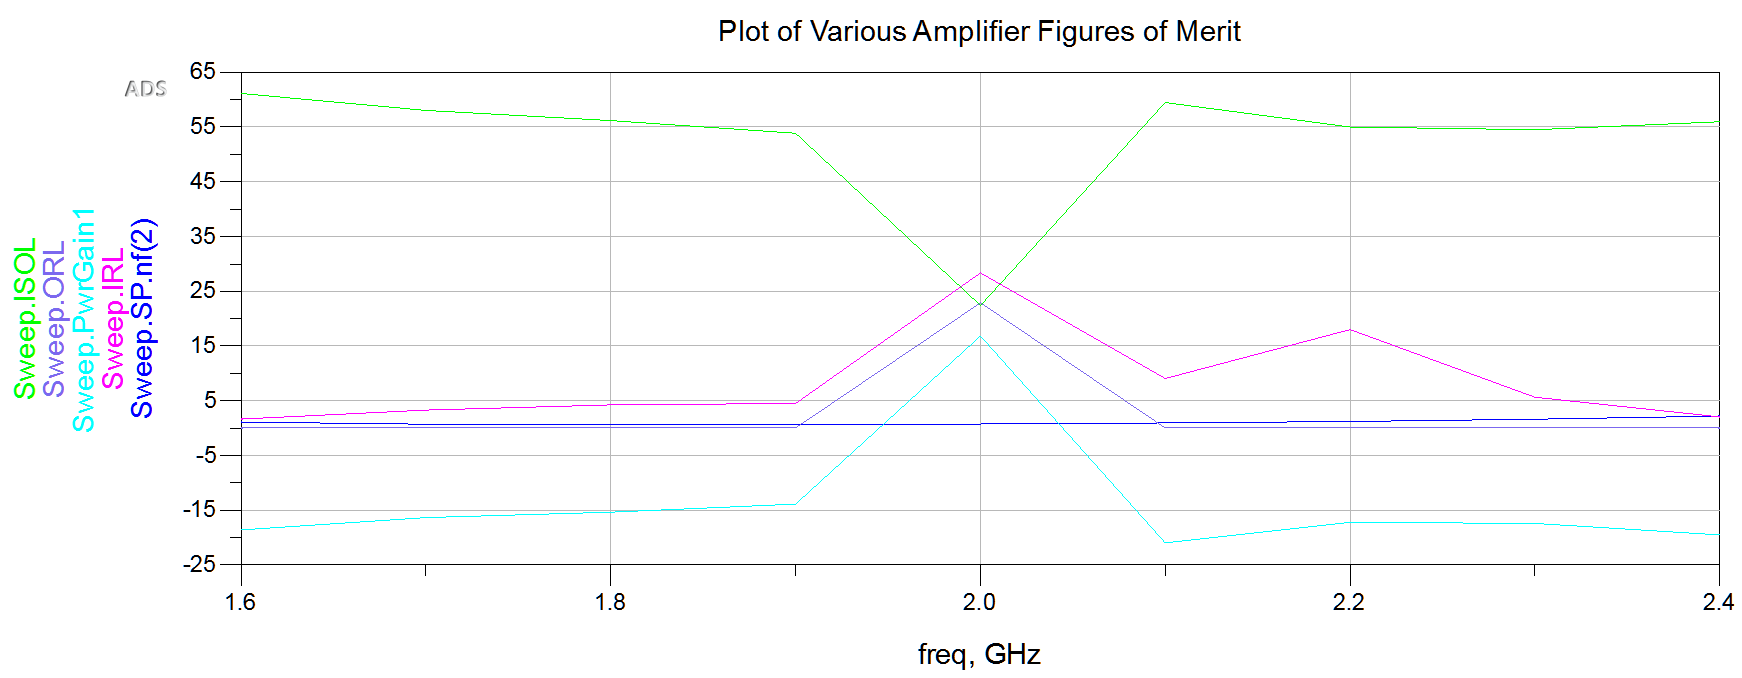
\includegraphics[width=0.8\linewidth]{Images/A2P2LNAFOM.png}
    \caption{Plot of various figures of merit of the amplifier including:
    Isolation (green), output return loss (purple), power gain (teal), input
return loss (pink) and noise figure (blue)}
    \label{fig:A2P2LNAFOM}
\end{figure}


\section{Appendix}

\subsection{Mathematica Code: Matching}
The code included in the subsection ``Mathematica Code: Matching'' provides the
Mathematica code that was used to generate the ideal match. Note that this ideal
match was not always used. In the case of the high-gain amplifier it was chosen
to reduce the gain from the maximum gain by almost as much as was possible
($\approx \SI{1}{\deci\bel}$) to ensure the lowest noise figure as was possible.
However, the results given are for those of an ideal match. To be clear, a table
is provided at the end of the section that enumerates which length of stub must
be used and what length of line (after the stub) must be used. The length of
line between the load and the stub is immaterial since the line is matched to
the load such that $Z_{in} = Z_l$.

\subsubsection{High Gain Amplifier}

\subsubsection{Low Noise Amplifier}

\subsection{MATLAB Scattering Parameter Analysis}

\subsubsection{High Gain Amplifier}

\subsubsection{Low Noise Amplifier}

\end{document}
